\documentclass[imperial]{octavo}
\RequirePackage{graphicx}
\usepackage[margin=1cm,right=1.5cm,top=2cm]{geometry}
\usepackage{fp,caption,keyval,ragged2e,lipsum,verbatim,textsamples,expl3,multicol,amsmath}
\usepackage[T1]{fontenc}
\usepackage{libertine}

\makeatletter
\RequirePackage{lstdoc}
\RequirePackage{graphicx}

\usepackage[figurename=Figure.,
                  justification=RaggedRight, 
                  labelfont={bf, footnotesize}, 
                  textfont={footnotesize},position=bottom]{caption}
%% Version 0.1 
% From bound.sty by Sigitas Tolu\v sis
% \topoint#1#2
% ------------
%  Dimension #1 in any unit of measure converts to value in points
%  and defines it to macro #2
%
\def\topoint#1#2{%
  \@tempdimb=#1
  \@tempcnta=\@tempdimb
  \multiply\@tempcnta by10
  \divide\@tempcnta by18647 \advance\@tempcnta by1
  \multiply\@tempcnta by72 \divide\@tempcnta by2540
  \expandafter\def\expandafter#2\expandafter{\the\@tempcnta}}
% Example 
% One cm to points \topoint{1cm}{\fromtop}
% the dimension is now in \fromtop
% it does not print the pt
% \subsection{Generic helpers}
%
% \begin{macro}{\@nameundef}
%  This is the opposite to |\@namedef| which is offered by the \LaTeX\ kernel.
%  We use it to remove the definition of some commands and keyval options after
%  |\begin{document}| (to save \TeX\ memory) and to remove caption options defined
%  with |\captionsetup|\oarg{type}. (From caption package.
%    \begin{macrocode}
\providecommand*\@nameundef[1]{%
  \expandafter\let\csname #1\endcsname\@undefined}
%    \end{macrocode}
% \end{macro}
%
% This counter counts the records in all the  DBs used.
%    \begin{macrocode}
\newcommand*\img@thecounter{0}
%    \end{macrocode}
%    \begin{macrocode}
\newcommand*\img@stepcounter{%
  \@tempcnta\img@thecounter
  \advance\@tempcnta\@ne
  \xdef\img@thecounter{\the\@tempcnta}}
%    \end{macrocode}
% \end{macro}

% This counter counts the records in the DB.
%    \begin{macrocode}
\newcommand*\sets@thecounter{0}
%    \end{macrocode}
%    \begin{macrocode}
\newcommand*\sets@stepcounter{%
  \@tempcnta\sets@thecounter
  \advance\@tempcnta\@ne
  \xdef\sets@thecounter{\the\@tempcnta}}
%    \end{macrocode}
% \end{macro}


\newcounter{imgcounter}
\setcounter{imgcounter}{0}

%  This helper macro checks if the first argument is in the comma separated
%  list which is offered as second argument. So for example
%  \begin{quote}
%    |\pics@ifinlist{frank}{axel,frank,olga,steven}{yes}{no}|
%  \end{quote}
%  would expand to |yes|.
%    \begin{macrocode}
\newcommand*\pics@ifinlist{%
  \@expandtwoargs\pics@@ifinlist}
%    \end{macrocode}
%    \begin{macrocode}
\newcommand*\pics@@ifinlist[2]{%
  \begingroup
  \def\@tempa##1,#1,##2\@nil{%
    \endgroup
    \ifx\relax##2\relax
      \expandafter\@secondoftwo
    \else
      \expandafter\@firstoftwo
    \fi}%
  \@tempa,#2,#1,\@nil}%
%    \end{macrocode}
% \end{macro}
%
%
%
\def\removeduplicates#1#2{%
  \let\@temp#1%
  \begingroup\gdef#2{}%
  \@for\next:=\@temp\do
  {\@ifundefined{lstel@\next}
    {\xdef#2{#2,\next}%
     \expandafter\let\csname lstel@\next\endcsname\@empty}
    {}%
  }%
  \endgroup
  \expandafter\strip@comma#2\@nil#2}
 \def\strip@comma,#1\@nil#2{\def#2{#1}}

%\get@firstelement{\alist}

\global\newcounter{@tempct}

%% gets any element by number
\def\get@element#1#2{%
  \let\i\@empty%
  \setcounter{@tempct}{0}%
  \setcounter{@tempct}{1}%
  \@for\i:=#2\do{%
    \ifnum\the@tempct=#1
     \xdef\FirstElement{\i}%
    \fi%
\stepcounter{@tempct}%
}}


%   We create an empty DB with the provided name.
%    #1  reserved for option list to be added later on
%    #2  DB name
%    #3  default path

\newcommand\@createDB[3][]{%
       % creates an empty list to hold the image names
       \expandafter\def\csname#2\endcsname{}
      % default path for images
       \expandafter\def\csname#2@path\endcsname{#3}
 }  

%  create a getter for the path
\newcommand\getpath[1]{\@nameuse{#1@path}}
\newcommand\listDB[1]{\@nameuse{#1}}


\let\newDB\@createDB
%    \end{macrocode}
% \end{macro}

%	We use lists extensively to store the fields and indices of the database
% 	start by adding list manipulation macros
% 	add element and define the element macro
% 	This adds an element to list and keep the list sorted
%	These macros have been borrowed from listings. 

\long\gdef\AddElementToList#1#2#3{%
    \lst@lAddTo{#1}{#2,}
    \lst@BubbleSort{#1}
    %image name store
    \def\tempb{\expandafter\@gobble\string#1}

    \expandafter\def\csname\tempb @#2\endcsname{{#2}}
%    %\expandafter\gdef\csname\tempa#2@caption\endcsname{#3}
%    \gdef\setshortcaption\tempa##2##3{\expandafter\gdef\csname##1##2@shortcaption\endcsname{##3}}
 }
\def\getimagename#1#2{\@nameuse{#1@#2}}

\def\getcaption#1#2{\@nameuse{#1#2@caption}}



%% we create a DB

\@createDB{kattaca}{./kattaca/}
%
\AddElementToList{\kattaca}{1}{First Image caption}
\AddElementToList{\kattaca}{2}{Second Image caption}
\AddElementToList{\kattaca}{3}{Third Image caption}
\AddElementToList{\kattaca}{4}{Fourth Image caption}
\begin{document}


\listDB{kattaca}\\
\getpath{kattaca}\\
\getcaption{kattaca}{2}\\
\getimagename{kattaca}{4}

\def\tempa{\getimagename{kattaca}{4}}

\edef\fullpath{}
\g@addto@macro{\fullpath}{\getpath{kattaca}{4}}


\def\put@graphic#1#2{%
    \includegraphics[height=6.92cm, keepaspectratio]{\getpath{#1}#2}}

%% becarefull there should be no spaces in the list!
%% 

\newgeometry{left=0pt,right=0pt,top=0cm,bottom=0cm}

\def\putall#1{%
%\centering
\noindent \@for\next:=#1\do{%
    \includegraphics[height=6.92cm, keepaspectratio]{./kattaca/\next}\hskip1pt%
 }}

\def\newlist{%
\def\remove@last@comma##1{%
     \def\remove@last@comma@####1####2,\@nil{####1####2}%
     \expandafter\remove@last@comma@##1\@nil%
}%
\remove@last@comma{\kattaca}%
}

\expandafter\putall{1,2,3,4,5,6}





%% Author command
\let\addimageDB\AddElementToList



%%  get single image

\def\getgr#1#2{%
  \edef\tempz{\getpath{#1}{#2}}
  \includegraphics[0.45\textwidth]{\tempz}}



\gdef\foreach#1{%
   \edef\zz{\csname#1\endcsname}
   \@for \next:=\zz \do{%
   \getgr{#1}{\next}}
}





%% Define some lengths so that we can measure images
%% and image boxes and pagelayouts
\global\newlength\miniwidth
\global\newlength{\imageh}
\global\newlength{\imaged}
\global\newlength{\imagew}

%% Initialize the fbox parameters to opt
\fboxsep0pt
\fboxsep0pt
%% The graphic command simply sets up the correct paths and includes the
%% image, this might need to be left in a box for later usage
%% I will come back and change it later.
%% We definekeys to enable manipulation of various parameters
%% which we pass to image macros
%% KEY DEFINITIONS
\define@key{img}{width}[1cm]{\def\img@width{#1}}
\define@key{img}{height}{\def\img@height{#1}}
\define@key{img}{scale}{\def\img@scale{#1}}
\define@key{img}{offsetx}{\def\img@offsetx{#1}}
\define@key{img}{offsety}{\def\img@offsety{#1}}
\define@key{img}{border}{\def\img@border{#1}}
\define@key{img}{padding}{\def\img@padding{#1}}
\define@key{img}{style}{\def\img@style{#1}}
\define@key{img}{bottommargin}{\def\img@bottommargin{#1}}
\define@key{img}{keepaspectratio}{\def\img@keepaspectratio{keepaspectratio}}
\define@key{img}{align}{\def\img@align{#1}}

%\define@key{imgpg}{pagestyle}{\def\imgpg@pagestyle{{#1}\centering}
%% Set defaults for all keys
\setkeys{img}{offsetx=1sp, offsety=0pt,width=0cm,height=0cm, 
                      border=0pt, padding=0pt,bottommargin=0pt,scale=1, align=0}
%% Create the command graphic
\newlength\tempc

%% We create a new command to place images 
%% #1 default holds all the keys
%% #2 filename
%% #3 holds caption - leave empty to ignore the caption
%% #4 How about inserting it as a key?

\newcommand\putimage[3][]{%
%% Set the keys
\setkeys{img}{#1}%
\setlength\fboxrule\img@border%
\setlength\fboxsep\img@padding%
\ifdim\img@offsety=0pt% 
   \else%
     \vspace*{\img@offsety}%
\fi%
\hskip\img@offsetx%
\setlength{\tempc}{\img@width}%
\def\setcaption{\captionof{figure}{#3}}%
\fbox{%
%% need to do calculations
%% First we calclulate the width and size of the 
%% image in order to arrange the enclosing box checks and dimensions
\let\outerbox\minipage%
\let\endouterbox\endminipage%
\parindent0pt%
\setlength{\miniwidth}{\img@width}
 \ifnum\img@align=0\centering \fi
\begin{outerbox}[b]{\miniwidth}%
     \fbox{%
        \begin{minipage}{\textwidth}%
           \vskip0pt
           \def\test{}%
          \ifdim\img@height>0pt%
              \g@addto@macro{\test}{height=\img@height,}% 
           \fi%

           \ifdim\img@width>0pt
                \g@addto@macro{\test}{width=\miniwidth,}% 
                \ifdim\img@height>0pt
                   \g@addto@macro{\test}{width=\miniwidth, keepaspectratio}% 
                \fi%
           \fi %
\noindent\fbox{\expandafter\includegraphics\expandafter[\test ]{#2}}%
 %% reset some of the values
 %% reset all keys
 \setkeys{img}{offsetx=0sp, offsety=0pt,width=0cm,height=0cm,%  
                      border=0pt, padding=0pt,bottommargin=0pt,scale=0,align=0}%
 \end{minipage}%%
}
\captionof{figure}{#3}%
\end{outerbox}}%
}

\newcommand\articleheading[1]{%
    \par
    \vspace*{2\baselineskip}
    \bgroup
    \LARGE\bf\textsf{\noindent #1}
    \egroup
   \vskip2\baselineskip
}

%% We define a command for second page notes

\def\coverpage#1{%
  \parindent0pt
  \putimage[width=1.16\textwidth,offsetx=-1.2cm, offsety=3\baselineskip, border=0pt,padding=0pt]{#1}{}\par
  \addvspace{3\baselineskip}
   \hbox to \hsize{\Huge \hfill\hfill{\MakeUppercase{\bf \textsf{\LaTeXe\ Images}}}}
   \vspace*{0.3cm}
   \hbox to \hsize{\Huge \hfill\hfill{\MakeUppercase{\bf \textsf{The Aspiring Hackers' Guide}}}}
  \vspace*{3\baselineskip}
   \hbox to \hsize{\huge \hfill\hfill\textsf{\hbox{Yiannis Lazarides}}} 
   \vfill\vfill
   \hbox to \hsize{\huge \hfill\hfill\textsf{\hbox{Published by Camel Press}}}
  \clearpage
}



\long\def\secondpage{\clearpage\null\vfill\vfill
\pagestyle{empty}
\begin{minipage}[b]{0.9\textwidth}
\footnotesize\raggedright
\setlength{\parskip}{0.5\baselineskip}
Copyright \copyright 2010--\the\year\ Dr Yiannis Lazarides\par
Permission is granted to copy, distribute and\slash or modify this document under the terms of the GNU Free Documentation License, version 1.2, with no invariant sections, no front-cover texts, and no back-cover texts.\par
A copy of the license is included in the appendix.\par
This document is distributed in the hope that it will be useful, but without any warranty; without even the implied warranty of merchantability or fitness for a particular purpose.
\end{minipage}
\vspace*{2\baselineskip}}


\usepackage{doccommands,logos,abbreviations}


\makeatother

\begin{document}
\restoregeometry
\newpage

\coverpage{cockfight}
\clearpage
\secondpage
\mainmatter


\begin{minipage}{\textwidth}
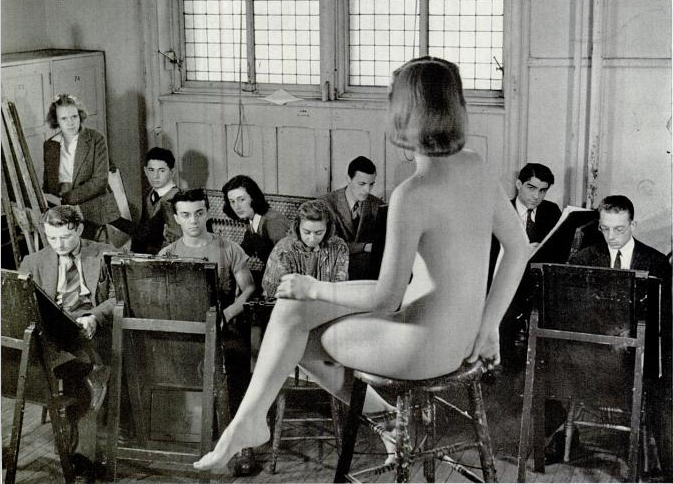
\includegraphics[width=\textwidth]{yaleartschool}
\articleheading{TRADITION AND TECHNIQUE AT YALE'S SCHOOL OF  FINE ARTS}
\end{minipage}
\begin{multicols}{3}
        \noindent\textbf{L}\lipsum*[1-2]
        \par
\end{multicols}


%%% CREATE DB FOR KATHLEEN PAINTINGS
% create the newDB
\newDB{kathleen}
% add images to the DB

\addimageDB{\kathleen}{napoleon}{Napoleon painting restored}
\addimageDB{\kathleen}{woman}{Napoleon painting restored}
\addimageDB{\kathleen}{pierced}{Napoleon painting restored}


\kathleen


\makeatletter
\@namedef{kathleen@napoleon}
%Filename \expandafter\includegraphics{\kathleen}
%\noindent\putimage[width=\textwidth,border=0pt,align=0]{\kathleennapoleon}{This is a short caption test and this one is a long caption test.}
\pagebreak




\pagebreak
\lipsum[1]
\putimage[height=0.8\textheight, width=\textwidth, offsetx=0cm,offsety=0cm,border=0pt]{nino}{This is a short caption test and this one is a long caption test.}

\putimage[width=\textheight, width=\textwidth, offsetx=0cm,offsety=0cm,border=0pt]{woman}{Donna Velata.}


\flushleft

\noindent\putimage[width=\textwidth,border=0pt]{odalisque}{This is a short caption test and this one is a long caption test.}
\vspace*{2\baselineskip}

\noindent\putimage[width=0.3\textwidth,border=0pt,align=1,border=0pt]{ginerva}{This is a short caption test and this one is a long caption test.}
%
%\begin{minipage}[b]{0.6\textwidth}
{\vskip-7.4cm
\leftskip0.41\textwidth
\noindent\textbf{\Huge \hfill Kathleen Gilje\hfill}\\[2\baselineskip]
\lipsum[7]\lorem
}
\pagebreak


\noindent\putimage[width=\textwidth,border=0pt,align=0,border=0pt,align=0]{napoleon}{This is a short caption test and this one is a long caption test.}

\leftskip2cm
\lipsum


\begin{minipage}[b][\textheight]{4.5cm}
%\vrule height4cm width1cm % aligns pictures on top! This is short of a miracle:)
\noindent\putimage[width=\textwidth,border=0pt,align=1,border=0pt]{ladyagnew}{This is a short caption test and this one is a long caption test.}
\noindent\putimage[width=\textwidth,border=0pt,align=1,border=0pt]{etta}{This is a short caption test and this one is a long caption test.}
\noindent\putimage[width=\textwidth,border=0pt,align=1,border=0pt]{etta}{This is a short caption test and this one is a long caption test.}
\end{minipage}\hspace{1cm}
\begin{minipage}[b][\textheight]{0.46\textwidth}
\noindent\putimage[width=\textwidth,border=0pt,align=1,border=0pt]{ladyagnew}{This is a short caption test and this one is a long caption test.}
\noindent\putimage[width=\textwidth,border=0pt,align=1,border=0pt]{etta}{This is a short caption test and this one is a long caption test.}
\end{minipage}

%\newgeometry{left=1cm,right=1cm}

\pagebreak

\chapter{MEASURING IMAGES AND BOXES}

\parindent0.5em

{using an image box}

It is important during automatic image placements to create page layouts to be able to measure the dimensions of an image automatically. This can be achieved by placing the contents of the page or section of a page in a box and then find the dimensions.

We begin by defining a temporary macro to hold the box contents.

\begin{verbatim}
\newcommand\testbox{%
    \begin{minipage}[b][\textheight]{0.46\textwidth}
        \noindent\putimage[width=\textwidth,border=0pt,align=1,border=0pt]{ladyagnew}{A caption.}
        \noindent\putimage[width=\textwidth,border=0pt,align=1,border=0pt]{etta}{A caption.}
    \end{minipage}%
}
\end{verbatim}


\newlength\graphicheight
\newlength\graphicwidth
\newcommand\testbox{\begin{minipage}[b][\textheight]{0.46\textwidth}
\putimage[width=\textwidth,border=0pt,align=1,border=0pt]{ladyagnew}{A caption.}
\putimage[width=\textwidth,border=0pt,align=1,border=0pt]{etta}{A caption.}
\end{minipage}}
\setlength\graphicheight{\heightof{\testbox}}
\setlength\graphicwidth{\widthof{\testbox}}
\the\graphicheight
\the\graphicwidth
\FPdiv\aspect{708.47363}{217.26842}
\FPmul\aspect{\aspect}{1}
\aspect
We will use \verb+\heightof+ and \verb!widthof! from the \texttt{calc} package to find out the dimensions.

\begin{verbatim}
\setlength\graphicheight{\heightof{\testbox}}
\setlength\graphicwidth{\widthof{\testbox}}
\end{verbatim}

\begin{verbatim}
\the\graphicheight
\the\graphicwidth
\end{verbatim}

Strip point \expandafter\strip@pt\graphicwidth

\subsection{Aspect ratio}
We define the aspect ratio as the ratio of the width of the image divided by the height. By determing the aspect ratio, we can then decide if the image can be placed in rows or columns for example.
\newcommand\aspectratio{\expandafter\the\numexpr((\graphicheight)/(\graphicwidth))}

To calculate the ratio, we will use the \texttt{fp} package.

\begin{verbatim}
\FPdiv\aspect{708.47363}{217.26842}
\FPmul\aspect{\aspect}{1}
\end{verbatim}
\FPdiv\aspect{708.47363}{217.26842}
\FPmul\aspect{\aspect}{1}
\aspect
\setlength\@tempdima{\aspect pt}
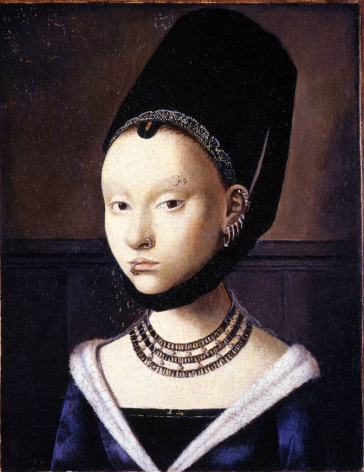
\includegraphics[width=25\@tempdima]{pierced}


\end{document}


http://www.artesmagazine.com/2010/07/new-york-artist-kathleen-gilje-revisits-john-singer-sargent%E2%80%99s-portraits-2/
http://kathleengilje.com/artwork/321569_Portrait_of_a_Lady_Restored_Pierced.html
\usepackage{calc}
...
\def\mygraphic{\includegraphics{...}}

\newlength\graphicheight
\setlength\graphicheight{\heightof{\mygraphic}}
% OR: \settoheight\graphicheight{\mygraphic}
